% !TeX root = ../main.tex
% Add the above to each chapter to make compiling the PDF easier in some editors.

\chapter{Implementation}\label{chapter:implementation}

The following chapter describes how the design discussed in \autoref{chapter:design} was implemented to function as a LAIK backend.
At first we will discuss the overall structure of the implemented backend.
We will then explain how the secondary backend version can be integrated into other backends.
The rest of the chapter will explain in detail how the previously discussed core functionality of the backend was implemented.

\section{Structure}

As we implement both a LAIK backend as well as the corresponding shared memory based communication library we split our backends functionality up into 2 files.
The first one implements the backend functionality and the second one the communication library for the backend.
The backend file (\code{backend-shmem.c}) will contain both the standalone version and the secondary backend version.
The standalone version has a similar structure to the MPI backend but it replaces all MPI library calls with equivalent ones to the shared memory library.
The secondary version part of this file provides a customized initialization routine for the secondary backend we will further discuss in \autoref{section:secondary_initialization}, an optimization pass to replace normal methods with shared memory based methods, an execution method to execute the shared memory actions and a finalize method which closes all open shared memory segments.
Those methods provide an interface which a developer can use to provide shared memory support for his primary backend.
The file providing the shared memory based communication library (\code{shmem.c}) implements the initialization routines and the data transport.

\subsection{Integration of the Secondary Backend Version in a Primary Backend}\label{section:integration}

As mentioned, the secondary backend version should be easily integratable into other backends.
To integrate the shared memory backend into a new backend a developer needs to amend the initialization, prepare and finalize methods of his backend.

The initialization method of the primary backend must call the modified secondary backend initialization routine to initialize the secondary backend.
As we discussed in \autoref{section:init_multiple_clusters}, the secondary initialization method needs to communicate with the primary backends communication library to discover processes on other nodes.
The primary backend therefore has to provide a send and receive function using its communication library.
Those two functions get passed as function pointers to the secondary backends initialization method. 

The primary's prepare method must be extended to also include the optimization pass of the shared memory backend.
The added optimization pass will replace generic actions with shared memory actions where possible.
As the added optimization pass introduces new shared memory backend specific methods, the primary's exec function needs be able to execute those.

The exec function must be changed, so that it calls the secondary exec function if it does not know how to execute a function.
The secondary exec function will then execute the action and return a success or, if it can not execute it return a failure.

To close all open shared memory segments, the primary's finalize must also calls the secondary backends finalize method.


\section{Initialization}

This section will first discuss how the general initialization mechanism was implemented.
After that we will explain the initializations differences between the standalone and the secondary backend version.

As we discussed in \autoref{section:initialization} we need to let every process try to create an exclusive shared memory segment to assign one process the rank of master.
The processes will try to create the segment by calling \code{shmget()} with a predefined value as \code{key} and the flags \code{IPC\_CREAT} and \code{IPC\_EXCL} set.
That way only the first process will succeed and all others will receive $-1$ from \code{shmget()}.
The master will then initialize a counter in the shared memory segment by setting an atomic integer to $0$.
The other processes which were not successful in creating the exclusive segment will then call \code{shmget()} again but without the \code{IPC\_EXCL} flag set.
They will then increment the atomic counter and assign themselves the counters value as rank.

After the ranks are assigned, each process will create a shared memory segment which will be needed for the data transport.
We will discuss those segments in more detail in \autoref{section:data_transport}.

\subsection{Standalone Initialization}

As the standalone version can only be deployed on one node, the environment variable \code{LAIK\_SIZE} can be used to determine the size of the shared memory cluster.
\code{LAIK\_SIZE} represents the number of processes of a running LAIK application.
The master will keep the exclusive shared memory segment open as long as the counters value is below \code{LAIK\_SIZE}.
After that every process will have gotten his rank and the initialization process can be ended.

\subsection{Secondary Initialization}\label{section:secondary_initialization}

As the secondary backend version can be deployed across multiple nodes, there can be multiple clusters.
After initialization each process needs to know which processes are in his cluster and what other processes exist.
As \code{LAIK\_SIZE} only depicts the number of all processes of a LAIK application it can not be used to determine the cluster size.

To compute the clusters we therefore introduce the concepts of primary and secondary ranks and colours.
A processes primary rank is the rank he has in the primary backends communication library.
The secondary rank is the rank the process got assigned himself during the secondary backend initialization.
Unlike the rank of the secondary backend, the rank of the primary backend is unique.
The colour of a process is the primary rank of the clusters master.
The colour therefore serves as an identifier for a cluster.
According to our definition, the processes seen in the exemplary LAIK application from \autoref{fig:example_application} result in the ranks and colours seen in \autoref{tab:ranks_and_colours}.

\begin{figure}[h]
	\centering
	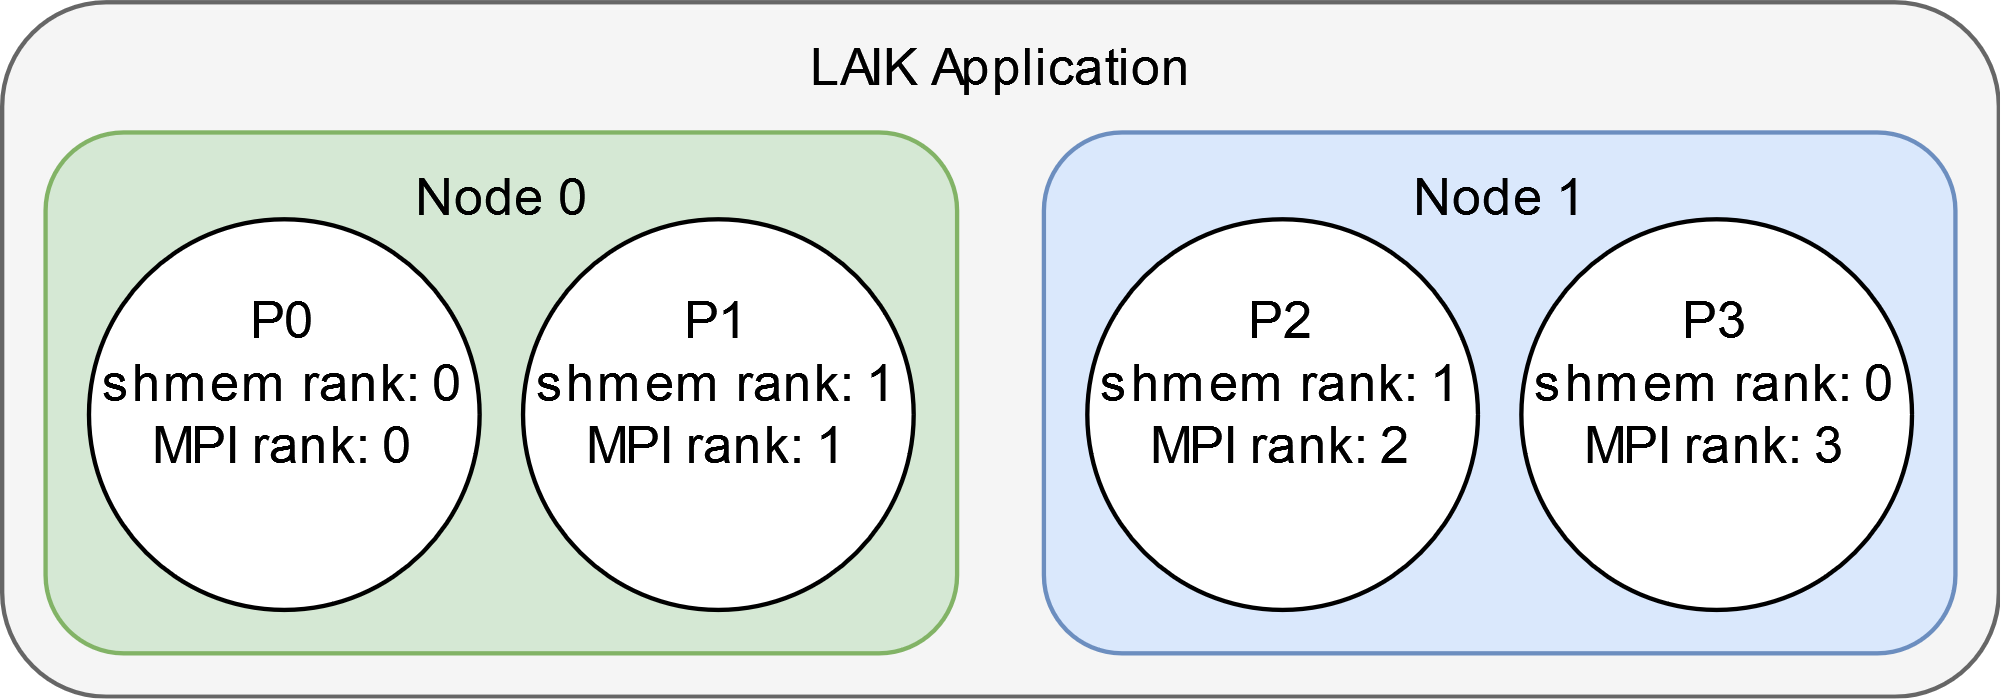
\includegraphics[width=0.66\columnwidth]{figures/example_application.png}
	\caption{Ranks of a LAIK application with 4 processes deployed on 2 nodes}
	\label{fig:example_application}
\end{figure}

\begin{table}[htpb]
	\centering
	\begin{tabular}{l l l l l}
		\toprule
		               & P0 & P1 & P2 & P3 \\
		\midrule
		primary rank   & 0  & 1  & 2 & 3   \\
		secondary rank & 0  & 1  & 1 & 0   \\
		color          & 0  & 0  & 3 & 3   \\
		\bottomrule	
	\end{tabular}
	\caption[Values of the example LAIK application]{The ranks and colours of the LAIK application from \autoref{fig:example_application}.}
	\label{tab:ranks_and_colours}
\end{table}

After each process got its rank from the atomic counter, they will then use the provided send and receive methods from the primary backend to send their secondary rank to the process with the primary rank 0.
This process will then accumulate all the nodes secondary ranks.
It will then compute the colour of every process and the sizes of all clusters and distribute that information to all the other nodes.
After that is done, every process knows which processes are in his group and what other processes exist.

\section{Data Transport}\label{section:data_transport}

This section explains how the data transport was implemented in \code{shmem.c}.
We will first explain how we decide which variant executes a given data migration.
After that, we will elaborate on the implementation of our 1 and 2 copy data transport versions.

To provide information about the shared memory segment which is about to be sent, each process has a semaphore to synchronize its sending operations and its own shared memory segment which hosts a \code{metaInfos} struct.
The \code{metaInfos} struct contains the receiving processes secondary rank, the number of elements to be sent, the shmid of the shared memory segment which is to be copied from as well as the offset the pointer has from the start of the shared memory segment.
The semaphore will be locked by the process it belongs to until he has completed a sending operation and waits for the receiving process to receive the data.
After the receiving process received the segment, the sending process will lock the semaphore again.

As discussed in \autoref{section:design_data_transport} the 2 copy version should only be used if an application directly provided memory.
All other \code{Laik\_Data} was allocated via a \code{Laik\_Allocator} and is therefore shared memory.
Every time a shared memory segment is allocated with via an allocator, the shared memory library saves the pointer to the segment, its shmid and its size.
This allows us to determine whether a given pointer points to a shared memory segment or not.
When a shared memory action gets executed, the one copy methods get called.
The 1 copy send method will then try to determine the shmid of the segment the given pointer points to.
If the given pointer to does not lie in any of the previously allocated shared memory segments, the sending process will set the shmid in the \code{metaInfos} struct to $-1$ and call the 2 copy version.
After the receive call reads the shmid out of the meta info segment it will check whether a valid shmid was given.
If the given shmid is $-1$ it will call the 2 copy version.

\subsection{2 Copy Transport}

As the 2 copy transport needs to create its own shared memory segment to copy the data to, it needs to generate a unique key for each transaction.
To generate this key we hash the secondary rank of the sender add the recipients rank and hash the sum again (\code{key = hash(rank\_recipient + hash(rank\_sender))}).
Those keys are unique for our purposes, since we can only have one send and receive operation between two processes at a time.
With the generated key the two processes create and open a shared memory segment which equals the buffers size.
The sending process will then copy his data into the segment and update his meta information segment.
After that he will unlock the semaphore for his segment.
The receiving process will then lock the semaphore and copy the data from the segment to its buffer.
After copying the data, the receiving process will free the semaphore which the sending process will immediately lock again. 

\subsection{1 Copy Transport}

The 1 copy transport is used if the given buffer pointer points to a shared memory segment.
The 1 copy send method will update the meta info segments information with the data of the new segment and free the semaphore.

As mentioned in \autoref{section:shared_memory} shared memory is mapped to each attached processes address space.
This means a pointers adress can differ between processes despite them pointing to the same element of a shared memory segment.
We therefore need to compute the pointer from the shared segments id and the offset which are accessible over the meta Information segment.
The offset is the difference between the pointers address and the shared segments address.  
To compute the actual pointer we first attach the shared memory segment by its id.
The offset must then be added to the returned pointer to compute the correct pointer.

After the sending operation unlocked the semaphore, the receiver is able to lock the semaphore and access the sending processes meta information segment.
The receiving process will then read shmid, offset and the sending operations number of elements.
The receiver will then check that his receiving buffer is big enough for all the data the sending process wants to send.
It will then copy the data directly from the sending processes buffer to its buffer.
The semaphore will then be unlocked by the receiving process and the sending process will lock the semaphore again. 


\section{Action Substitution}

In this section we will elaborate on how the generic actions get replaced by shared memory actions.

Every action has a type which is an unique integer to identify the action.
We defined our own action types four our shared memory actions.
To replace the generic actions we need to change their type to the corresponding shared memory action type.

As mentioned in \autoref{section:integration} \code{backend-shmem.c} provides an optimization pass with the signature \code{bool laik\_aseq\_replaceWithShmemCalls(Laik\_ActionSeq *as)}.
This method replaces the generic actions with shared memory actions where possible by iterating over the actions and checking whether they can be replaced.

A generic call can be replaced when all involved processes are in the same cluster.
This can be determined by looking at the processes colour which identifies the cluster they are in.
If all processes have the same colour, the action type will be changed to the corresponding shared memory action type and the primary ranks stored in the action will be replaced by the corresponding secondary rank.
This ensures that the shared memory library can process the actions correctly.

\section{Action Execution}

We discussed in \autoref{section:integration} that the primary backend calls the secondary backend if it can not execute an action because its type is unknown to the primary backend.
In that case the method \code{bool laik\_shmem\_secondary\_exec(Laik\_ActionSeq *as, Laik\_Action *a)} is called to execute the action.
This method checks whether the given actions type is known to the secondary backend and executes it if it knows the type.
In that case the method returns true, if it does not know the action it returns false.
This is done to let the primary backend know whether the action was executed by the secondary or if it should alert LAIK due to an unknown action.